\begin{table}[H]
  \centering
  \caption{Correspondance entre objectifs spécifiques et choix méthodologiques}
  \label{tab:objectifs_choix_methodologiques}
  \tableStyleStart
  \begin{tabularx}{\textwidth}{p{4.1cm}X}
    \rowcolor{darkblue}
    \tabheader{Objectif spécifique} & \tabheader{Choix méthodologique retenu} \\
    \midrule
    Normaliser les offres, candidats et référentiels & Construction d'une couche de données standardisée : identifiants stables, champs nettoyés, niveaux de formation, secteurs, compétences et textes d'embedding. \\
    Adapter la recherche sémantique au domaine emploi-compétences & Fine-tuning contrastif d'un modèle SentenceTransformer, puis indexation des embeddings dans PostgreSQL avec pgvector pour le retrieval top-$K$ \cite{reimers2019sbert,pgvector2024}. \\
    Représenter les relations entre métiers, compétences et profils & Construction d'un graphe de connaissances Neo4j reliant candidats, offres, compétences, métiers, secteurs, localisations et référentiels \cite{hogan2021knowledge,hamilton2020graph}. \\
    Produire une recommandation explicable & Score hybride combinant similarité vectorielle, couverture de compétences, compatibilité de niveau et alignement sectoriel, complété par une analyse de \textit{skill gap}. \\
    Orchestrer la réponse utilisateur & Workflow LangGraph routant la requête vers les outils adaptés : pgvector, Neo4j, recherche documentaire, Text2Cypher, critic et génération finale. \\
    Evaluer la qualité du système & Protocole séparant l'évaluation du retrieval, du graphe, du classement et de la réponse générée. \\
    \bottomrule
  \end{tabularx}
  \tableStyleEnd
  \source{Nos travaux, traitements Python de nettoyage et de diagnostic, à partir des données collectées du projet.}
\end{table}

\begin{table}[H]
  \centering
  \caption{Volumes réellement exploités par les modules de recommandation}
  \label{tab:implementation_volumes_exploites}
  \tableStyleStart
  \begin{tabularx}{0.94\textwidth}{XrX}
    \rowcolor{darkblue}
    \tabheader{Objet exploité} & \tabheader{Volume} & \tabheader{Utilité pour le système} \\
    \midrule
    Offres normalisées & 13\,957 & Base principale à recommander, indexée dans pgvector et reliée au graphe. \\
    Candidats normalisés & 41\,298 & Vivier à partir duquel sont calculés les rapprochements offre--profil. \\
    Compétences indexées & 13\,939 & Signal de matching, de filtrage et de justification du \textit{skill gap}. \\
    Secteurs nettoyés & 1\,039 & Signal de contexte pour limiter les rapprochements absurdes entre domaines trop éloignés. \\
    Métiers indexés & 3\,039 & Niveau d'agrégation utile pour stabiliser les recommandations au-delà des intitulés d'offres. \\
    Groupes métiers MEPC & 209 & Référentiel externe pour structurer les proximités métier. \\
    Domaines détaillés NCF & 201 & Référentiel de formation utilisé pour contextualiser les niveaux et domaines. \\
    Localisations représentées dans Neo4j & 312 & Signal géographique pour filtrage souple et explication des résultats. \\
    \bottomrule
  \end{tabularx}
  \tableStyleEnd
  \source{Nos travaux, diagnostics PostgreSQL}
\end{table}

\begin{figure}[H]
  \centering
  \caption{Localisation nettoyée des offres}
  \label{fig:implementation_localisation}
  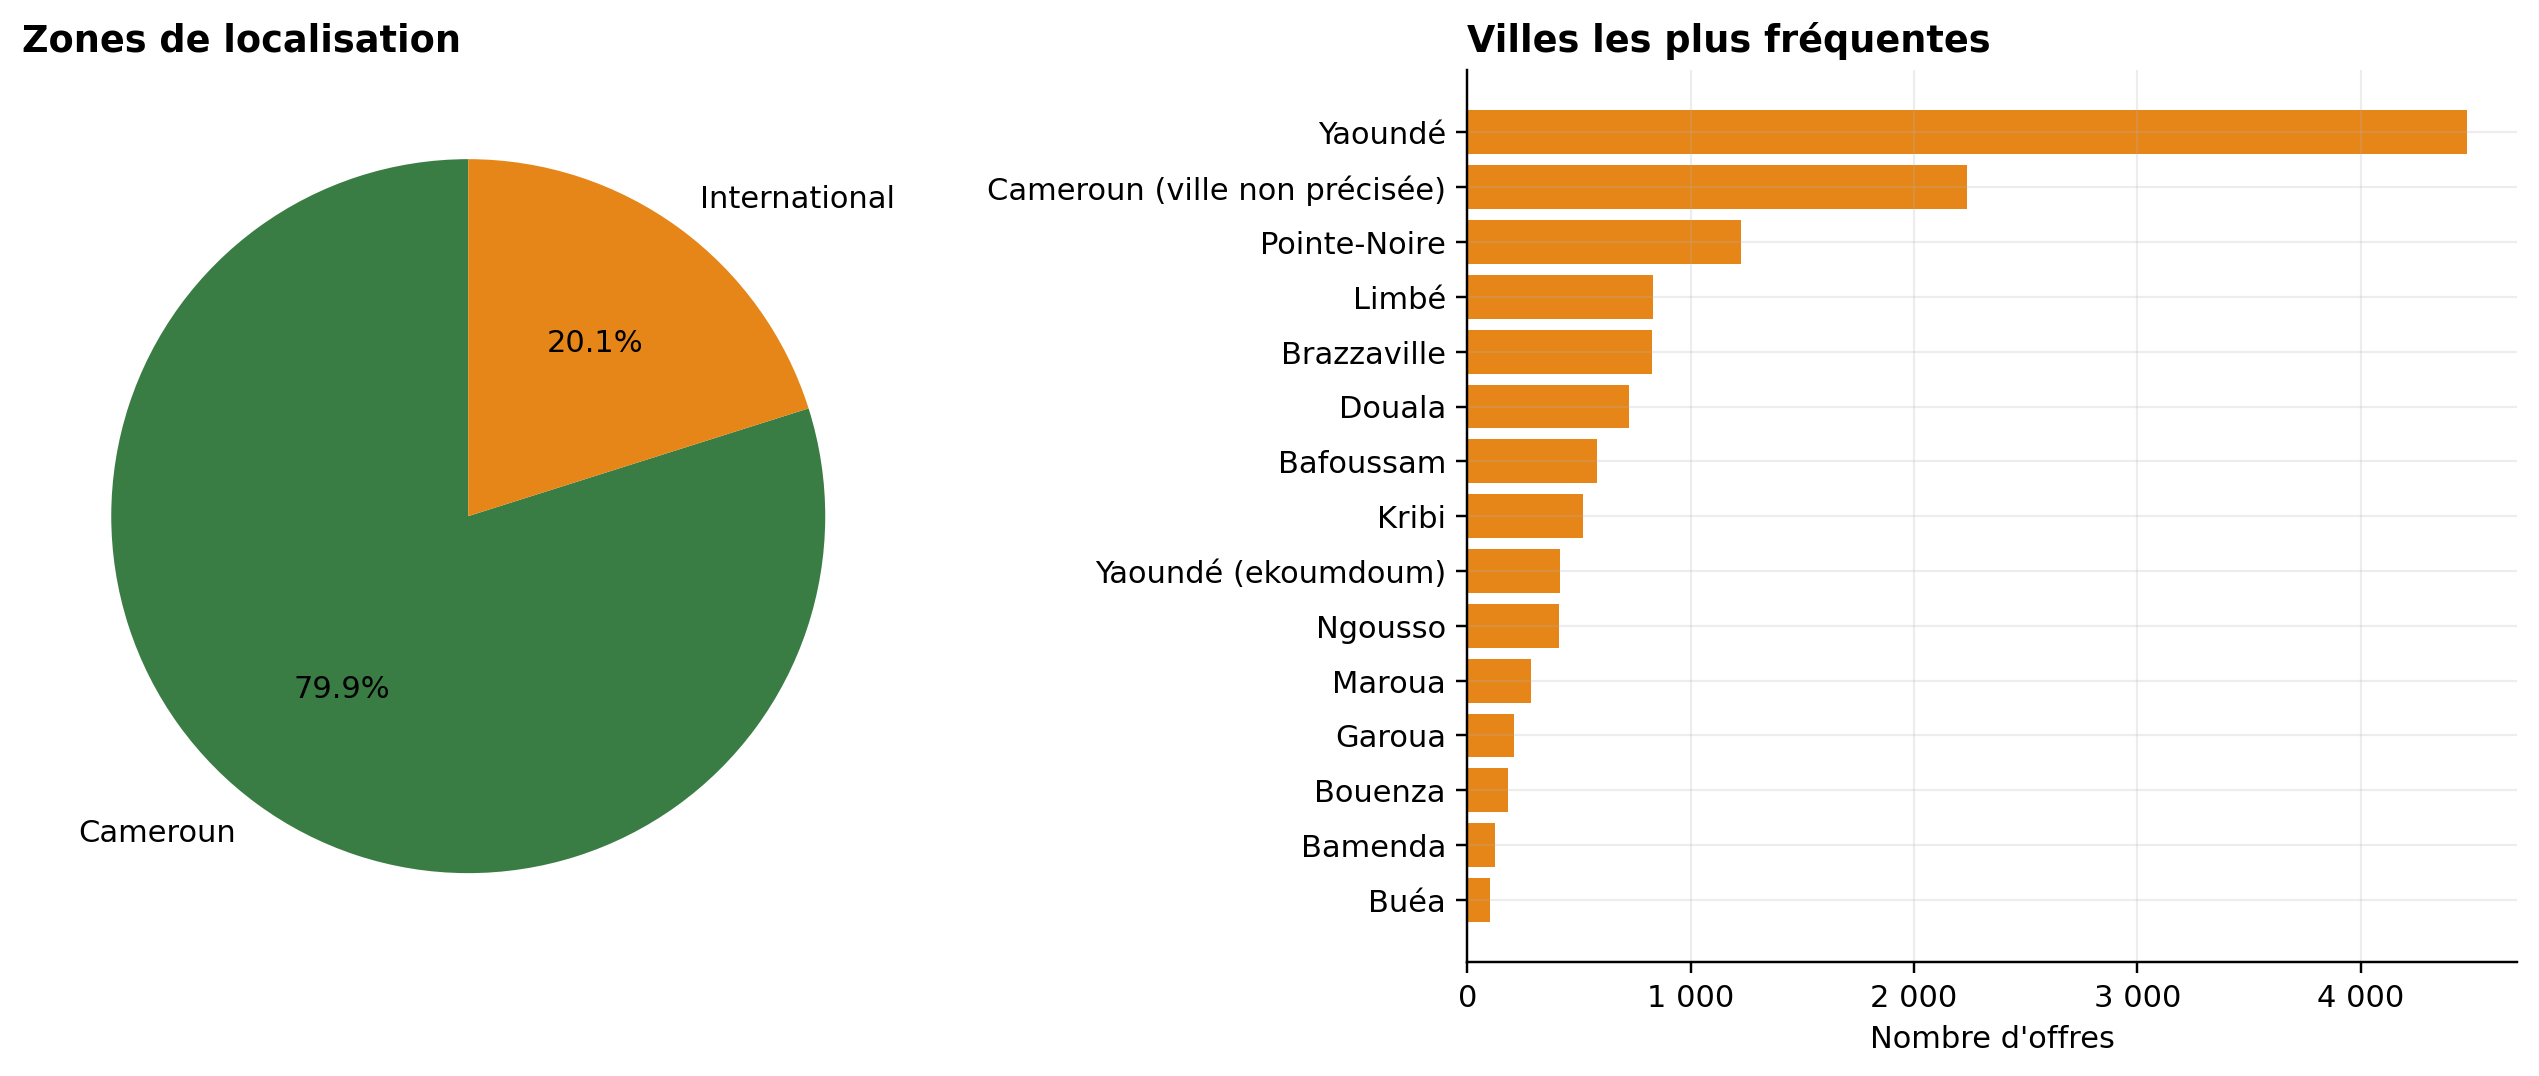
\includegraphics[width=0.94\textwidth]{figures/generated/implementation_deep_current/02_localisation_mixte.png}
  \source{Nos travaux, traitements Python de nettoyage et de diagnostic, à partir des données collectées du projet.}
\end{figure}

\begin{table}[H]
  \centering
  \caption{Synthèse des traitements de nettoyage utiles au moteur de recommandation}
  \label{tab:implementation_nettoyage_donnees}
  \tableStyleStart
  \begin{tabularx}{0.96\textwidth}{p{3.4cm}XX}
    \rowcolor{darkblue}
    \tabheader{Traitement} & \tabheader{Décision implémentée} & \tabheader{Effet attendu} \\
    \midrule
    Casse et formats & Harmonisation des libellés pour réduire les variantes d'écriture. & Moins de fragmentation dans les compétences, secteurs, villes et sources. \\
    Doublons & Validation uniquement si toute la ligne est identique sur toutes les variables. & Suppression prudente des répétitions exactes, sans effacer des offres proches mais distinctes. \\
    Localisation & Séparation Cameroun, international et non précisée ; conservation des localités fines disponibles. & Filtrage géographique possible sans perte des offres incomplètes. \\
    Champs vides & Modalités explicites lorsque le champ reste exploitable comme absence d'information. & Le système peut pénaliser ou contextualiser le manque d'information au lieu d'ignorer l'offre. \\
    Descriptions faibles & Enrichissement de la représentation par métadonnées et compétences. & Robustesse accrue pour les sources où le détail de l'offre est absent ou court. \\
    \bottomrule
  \end{tabularx}
  \tableStyleEnd
  \source{Nos travaux, traitements Python de nettoyage et de diagnostic, à partir des données collectées du projet.}
\end{table}

\begin{table}[H]
  \centering
  \caption{Comparaison directe entre le baseline et le modèle fine-tuné}
  \label{tab:implementation_baseline_vs_finetuned}
  \tableStyleStart
  \begin{tabularx}{0.86\textwidth}{Xrrr}
    \rowcolor{darkblue}
    \tabheader{Métrique test} & \tabheader{Baseline} & \tabheader{Fine-tuné} & \tabheader{Gain} \\
    \midrule
    NDCG@10 & 0,1681 & 0,6232 & +0,4552 \\
    MRR@10 & 0,1410 & 0,5874 & +0,4463 \\
    Recall@1 & 0,0986 & 0,5268 & +0,4281 \\
    Recall@5 & 0,1983 & 0,6632 & +0,4648 \\
    Recall@10 & 0,2560 & 0,7398 & +0,4837 \\
    Precision@1 & 0,0986 & 0,5268 & +0,4281 \\
    \bottomrule
  \end{tabularx}
  \tableStyleEnd
  \source{Nos travaux, traitements Python et SentenceTransformer}
\end{table}

\begin{table}[H]
  \centering
  \caption{Diagnostic statistique du chunking documentaire}
  \label{tab:implementation_pgvector_chunking}
  \tableStyleStart
  \begin{tabularx}{0.94\textwidth}{Xr}
    \rowcolor{darkblue}
    \tabheader{Indicateur} & \tabheader{Valeur observée} \\
    \midrule
    Documents sources indexés & 3 \\
    Chunks documentaires indexés & 142 \\
    Stratégie réellement utilisée & 100\,\% structurelle \\
    Taille moyenne & 187,1 tokens \\
    Taille médiane & 116,0 tokens \\
    Écart-type & 169,6 tokens \\
    Minimum / maximum & 6 / 492 tokens \\
    Coefficient de variation & 0,91 \\
    Chunks avec embedding & 142 / 142 \\
    Chunks synchronisés avec Neo4j & 142 / 142 \\
    \bottomrule
  \end{tabularx}
  \tableStyleEnd
  \source{Nos travaux, traitements Python de nettoyage et de diagnostic, à partir des données collectées du projet.}
\end{table}

\begin{table}[H]
  \centering
  \caption{Couverture documentaire et duplication des chunks}
  \label{tab:implementation_chunking_coverage_duplication}
  \tableStyleStart
  \begin{tabularx}{0.92\textwidth}{Xrr}
    \rowcolor{darkblue}
    \tabheader{Source} & \tabheader{Couverture approximative} & \tabheader{Chunks} \\
    \midrule
    NCF 2017 & 25,9\,\% & 38 \\
    MEPC 2013 & 23,6\,\% & 61 \\
    Référentiel des diplômes & 79,3\,\% & 43 \\
    \midrule
    Taux de duplication cosinus $>0{,}95$ & 0,0\,\% & 142 \\
    Similarité maximale hors diagonale & 0,921 & -- \\
    \bottomrule
  \end{tabularx}
  \tableStyleEnd
  \source{Nos travaux, traitements Python de nettoyage et de diagnostic, à partir des données collectées du projet.}
\end{table}

\begin{table}[H]
  \centering
  \caption{Cohérence sémantique intra-chunk}
  \label{tab:implementation_chunking_coherence}
  \tableStyleStart
  \begin{tabularx}{0.92\textwidth}{Xrrr}
    \rowcolor{darkblue}
    \tabheader{Source} & \tabheader{Moyenne} & \tabheader{Médiane} & \tabheader{Intervalle observé} \\
    \midrule
    MEPC 2013 & 0,307 & 0,288 & 0,191--0,502 \\
    NCF 2017 & 0,336 & 0,321 & 0,259--0,474 \\
    Référentiel des diplômes & 0,268 & 0,260 & 0,066--0,457 \\
    \bottomrule
  \end{tabularx}
  \tableStyleEnd
  \source{Nos travaux, traitements Python de nettoyage et de diagnostic, à partir des données collectées du projet.}
\end{table}

\begin{table}[H]
  \centering
  \caption{Indicateurs techniques pgvector}
  \label{tab:implementation_pgvector_indicateurs}
  \tableStyleStart
  \begin{tabularx}{0.92\textwidth}{Xr}
    \rowcolor{darkblue}
    \tabheader{Indicateur} & \tabheader{Valeur observée} \\
    \midrule
    Embeddings d'entités structurées & 72\,643 \\
    Chunks documentaires indexés & 142 \\
    Dimension des vecteurs & 384 \\
    Modèle d'encodage & \texttt{all-MiniLM-L6-v2-ft-offres-cm} \\
    Index PostgreSQL sur \texttt{embeddings} et \texttt{doc\_chunks} & 19 \\
    Taille totale de la table \texttt{embeddings} & 259,05 Mo \\
    Taille de l'index \texttt{emb\_hnsw} & 81,30 Mo \\
    Taille totale de \texttt{doc\_chunks} & 1,51 Mo \\
    Latence moyenne top-10 HNSW sur 25 requêtes & 34,31 ms \\
    Latence médiane top-10 HNSW sur 25 requêtes & 30,89 ms \\
    Latence p90 top-10 HNSW sur 25 requêtes & 64,41 ms \\
    \bottomrule
  \end{tabularx}
  \tableStyleEnd
  \source{Nos travaux, diagnostics PostgreSQL}
\end{table}

\begin{table}[H]
  \centering
  \caption{Index pgvector et index complémentaires}
  \label{tab:implementation_pgvector_index}
  \tableStyleStart
  \begin{tabularx}{\textwidth}{p{3.4cm}p{4.6cm}X}
    \rowcolor{darkblue}
    \tabheader{Famille d'index} & \tabheader{Index observés} & \tabheader{Usage dans le retrieval} \\
    \midrule
    Vectoriel HNSW & \texttt{emb\_hnsw}, \texttt{doc\_chunks\_hnsw} avec \texttt{vector\_cosine\_ops}. & Recherche approximative des plus proches voisins en similarité cosinus. \\
    B-tree métier & \texttt{emb\_offre\_idx}, \texttt{emb\_candidat\_idx}, \texttt{emb\_competence\_idx}, \texttt{emb\_metier\_idx}. & Filtrage par type d'entité et accès rapide aux objets métiers. \\
    Synchronisation graphe & \texttt{emb\_neo4j\_idx}. & Passage d'un résultat vectoriel vers le noeud Neo4j correspondant. \\
    Modèle et unicité & \texttt{emb\_model\_idx}, contrainte unique \texttt{entity\_kind, entity\_id, model\_id}. & Éviter les doublons d'embeddings et gérer les futures versions de modèles. \\
    Recherche lexicale & \texttt{emb\_fulltext\_fr\_idx}, \texttt{doc\_chunks\_fulltext\_fr\_idx}. & Complément lexical français pour requêtes par mots exacts, acronymes ou intitulés rares. \\
    Référentiels & \texttt{doc\_chunks\_ncf\_idx}, \texttt{doc\_chunks\_mepc\_idx}, \texttt{doc\_chunks\_source\_idx}. & Recherche ciblée dans NCF, MEPC et référentiel des diplômes. \\
    \bottomrule
  \end{tabularx}
  \tableStyleEnd
  \source{Nos travaux, diagnostics PostgreSQL}
\end{table}

\begin{figure}[H]
  \centering
  \caption{Composition du graphe par types de noeuds et relations}
  \label{fig:implementation_neo4j_composition}
  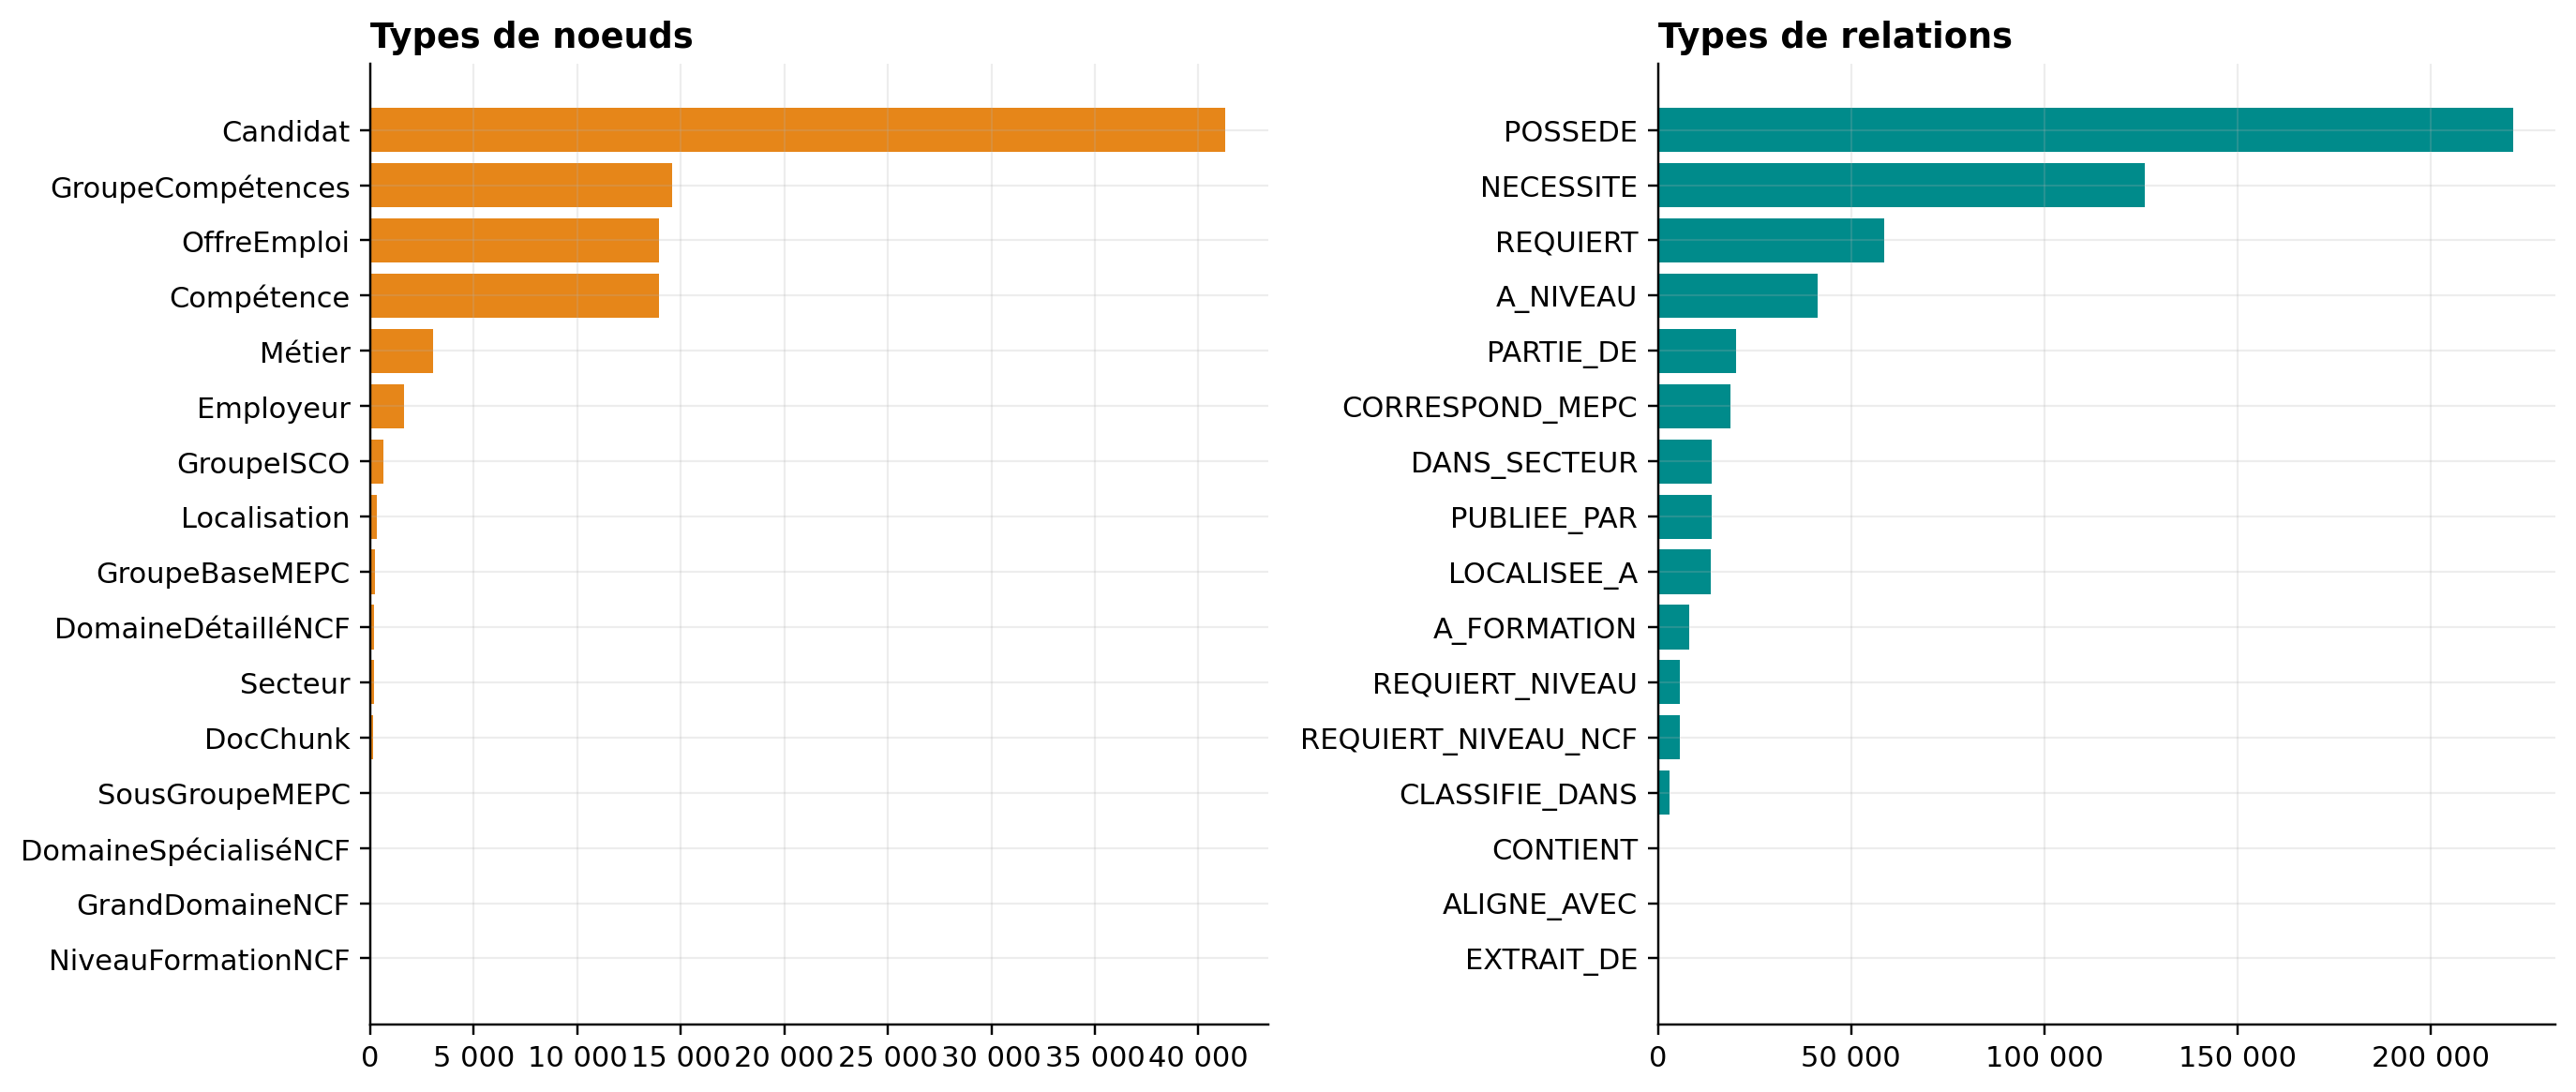
\includegraphics[width=0.55\textwidth]{figures/generated/implementation_deep_current/08_neo4j_composition.png}
  \source{Nos travaux, diagnostics Neo4j.}
\end{figure}

\begin{figure}[H]
  \centering
  \caption{Distribution des degrés dans la projection matching}
  \label{fig:implementation_neo4j_distribution_degres}
  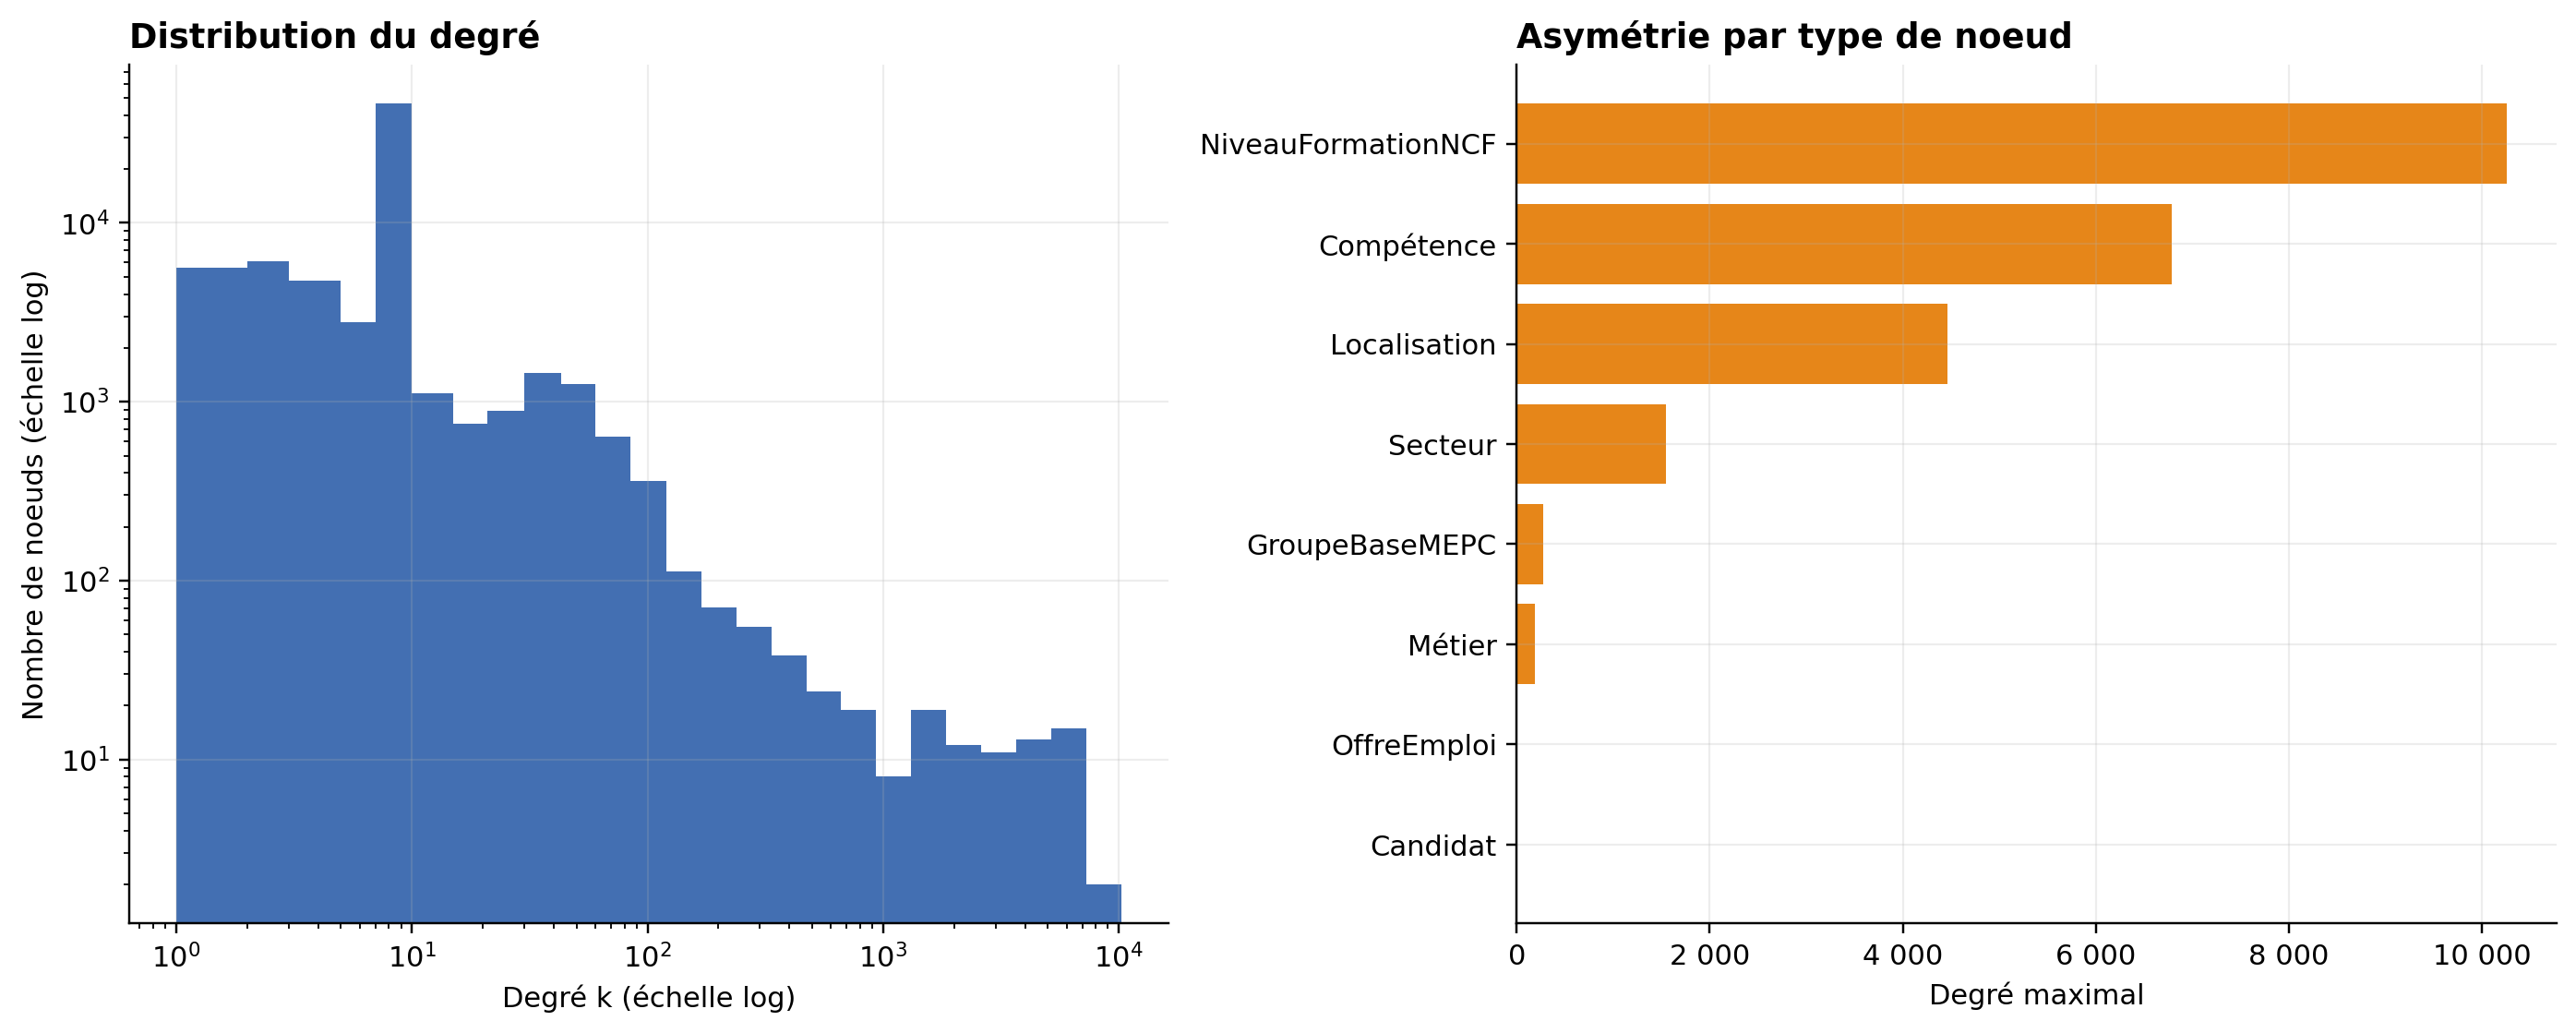
\includegraphics[width=0.55\textwidth]{figures/generated/implementation_deep_current/14_neo4j_distribution_degres.png}
  \source{Nos travaux, diagnostics Neo4j, à partir du graphe de connaissances emploi--compétences construit dans le projet.}
\end{figure}

\begin{table}[H]
  \centering
  \caption{Hétérogénéité des degrés par famille de noeuds}
  \label{tab:implementation_neo4j_degres}
  \tableStyleStart
  \begin{tabularx}{0.94\textwidth}{Xrrrr}
    \rowcolor{darkblue}
    \tabheader{Label} & \tabheader{Moyenne} & \tabheader{Médiane} & \tabheader{p90} & \tabheader{Max} \\
    \midrule
    \texttt{NiveauFormationNCF} & 5\,812,56 & 7\,073 & 10\,672,4 & 11\,050 \\
    \texttt{GroupeBaseMEPC} & 90,22 & 73 & 201 & 276 \\
    \texttt{Secteur} & 72,69 & 5,5 & 151,6 & 1\,548 \\
    \texttt{Métier} & 48,61 & 44 & 77 & 186 \\
    \texttt{Localisation} & 43,96 & 1 & 8 & 4\,467 \\
    \texttt{Compétence} & 30,57 & 5 & 28 & 6\,789 \\
    \texttt{OffreEmploi} & 7,97 & 9 & 11 & 11 \\
    \texttt{Candidat} & 6,56 & 7 & 8 & 8 \\
    \bottomrule
  \end{tabularx}
  \tableStyleEnd
  \source{Nos travaux, diagnostics Neo4j, à partir du graphe de connaissances emploi--compétences construit dans le projet.}
\end{table}
\begin{figure}[H]
  \centering
  \caption{Compétences par offre, candidat et métier dans Neo4j}
  \label{fig:implementation_neo4j_competences_entites}
  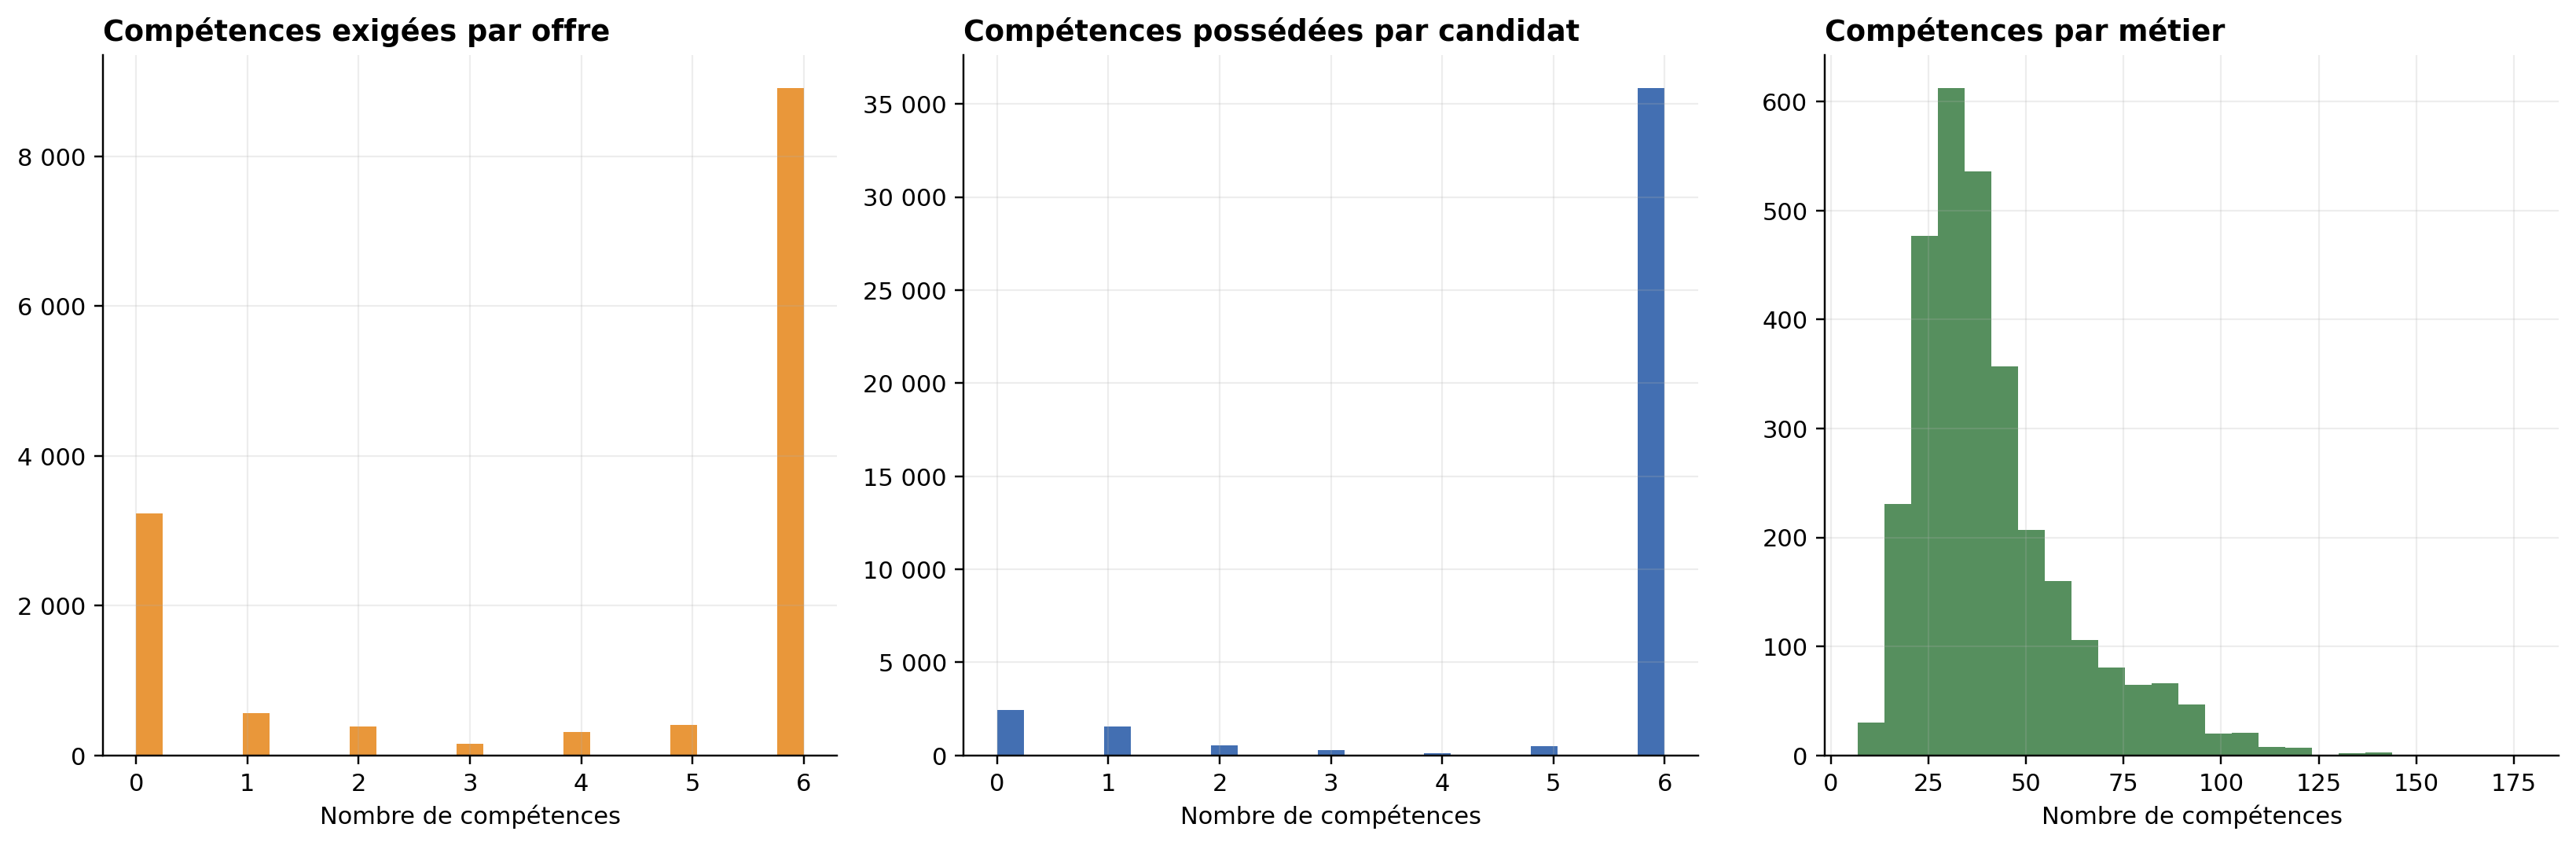
\includegraphics[width=0.55\textwidth]{figures/generated/implementation_deep_current/17_neo4j_competences_metier_offre_candidat.png}
  \source{Nos travaux, diagnostics Neo4j.}
\end{figure}

\begin{figure}[H]
  \centering
  \caption{Distribution échantillonnée du skill gap candidat--offre}
  \label{fig:implementation_neo4j_skill_gap}
  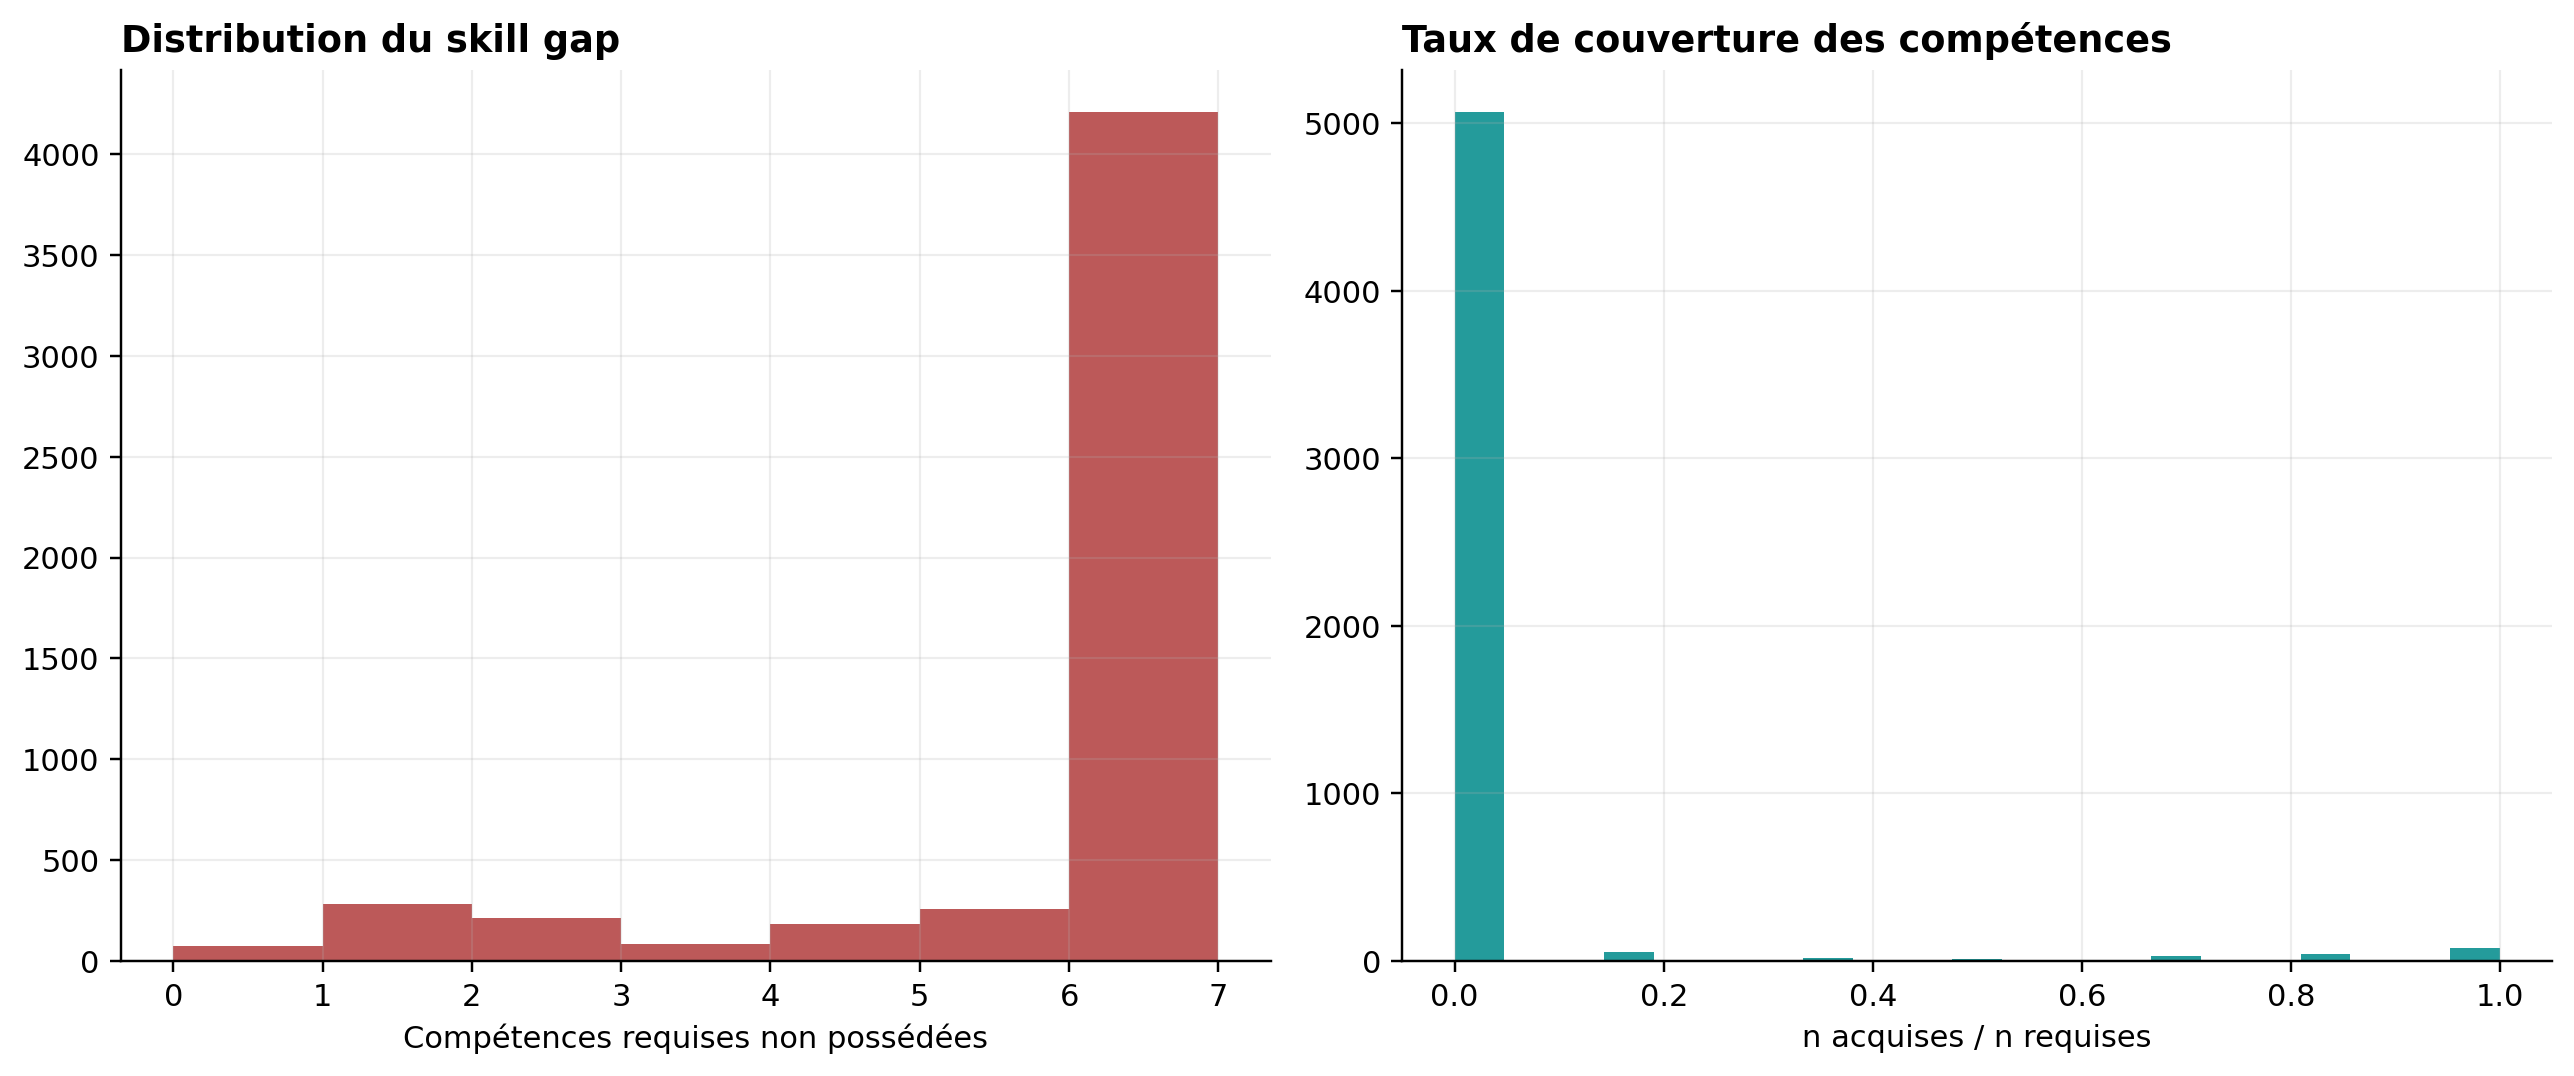
\includegraphics[width=0.55\textwidth]{figures/generated/implementation_deep_current/17_neo4j_skill_gap_distribution.png}
  \source{Nos travaux, diagnostics Neo4j}
\end{figure}

\begin{table}[H]
  \centering
  \caption{Résumé du déplacement de rang après reranking Neo4j}
  \label{tab:implementation_moteur_hybride_scores}
  \tableStyleStart
  \begin{tabularx}{0.92\textwidth}{Xr}
    \rowcolor{darkblue}
    \tabheader{Indicateur} & \tabheader{Valeur} \\
    \midrule
    Couples candidat--offre évalués & 690 \\
    Candidats distincts & 69 \\
    Rang moyen avant reranking pgvector & 9,51 \\
    Rang moyen après reranking Neo4j/Optuna & 5,50 \\
    Déplacement moyen de rang & +4,01 \\
    Déplacement médian & +1,00 \\
    Offres remontées & 59,86\,\% \\
    Offres rétrogradées & 13,77\,\% \\
    Offres inchangées & 26,38\,\% \\
    \bottomrule
  \end{tabularx}
  \tableStyleEnd
  \source{Nos travaux, traitements Python de nettoyage et de diagnostic}
\end{table}
